This benchmark is based on Thieulot \& Puckett [Subm.] in which an analytical solution to the
isoviscous incompressible Stokes equations is derived in an annulus geometry.
The velocity and pressure fields are as follows:

\begin{eqnarray}
v_r(r,\theta)     &=&  g(r) k \sin(k\theta), \\
v_\theta(r,\theta)&=&  f(r) \cos(k \theta), \\ 
p(r,\theta)       &=&  k h(r) \sin(k \theta), \\
\rho (r,\theta)   &=& \aleph(r) k \sin (k \theta), 
\end{eqnarray}
with
\begin{eqnarray}
f(r)&=&Ar+B/r, \\
g(r) &=& \frac{A}{2}r  +  \frac{B}{r} \ln r + \frac{C}{r}, \\
h(r)&=& \frac{2g(r)-f(r)}{r},  \\
\aleph(r) &=& g'' - \frac{g'}{r}  - \frac{g}{r^2} (k^2 - 1)  + \frac{f}{r^2}   + \frac{f'}{r}, \\
A &=& -C\frac{2(\ln R_1 - \ln R_2)} { R_2^2 \ln R_1  - R_1^2 \ln R_2}, \\
B &=& -C \frac{R_2^2-R_1^2}{R_2^2 \ln R_1 - R_1^2 \ln R_2}.
\end{eqnarray}

The parameters $A$ and $B$ are chosen so that $v_r(R_1)=v_r(R_2)=0$, i.e.
the velocity is tangential to both inner and outer surfaces.
The gravity vector is radial and of unit length.
In the present case, we set $R_1=1$, $R_2=2$ and $C=-1$. 

\fbox{
\parbox{10cm}{{\bf features}
\begin{itemize}
\item $Q_1\times P_0$ element
\item incompressible flow
\item penalty formulation
\item Dirichlet boundary conditions
\item direct solver
\item isothermal
\item isoviscous
\item analytical solution
\item annulus geometry
\item elemental boundary conditions
\end{itemize}
}}

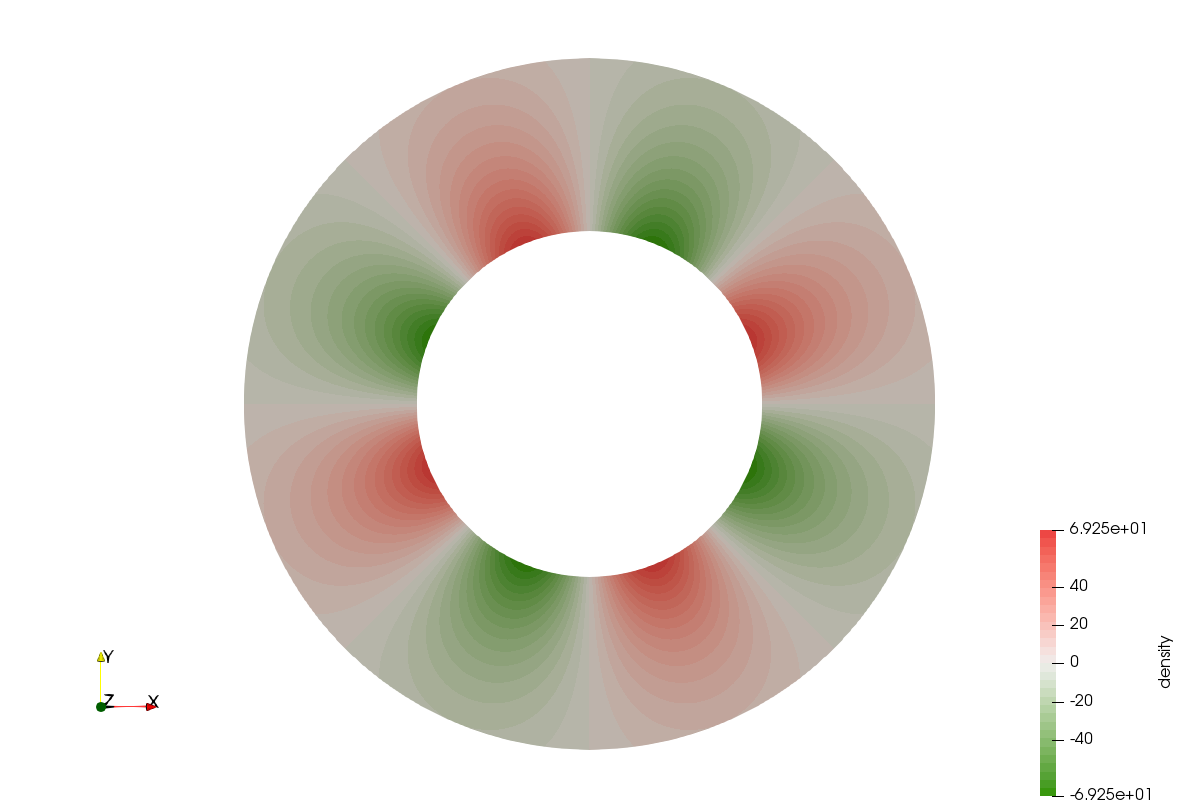
\includegraphics[width=6cm]{python_codes/fieldstone_09/density}
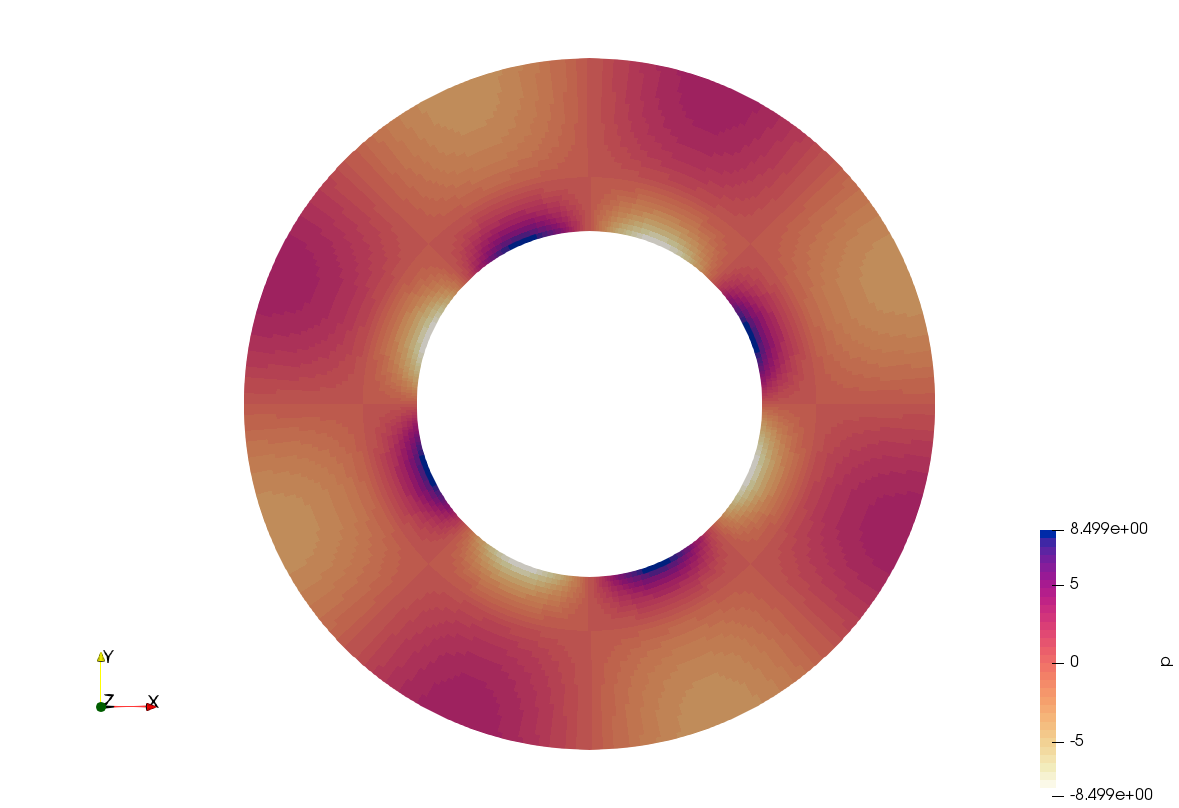
\includegraphics[width=6cm]{python_codes/fieldstone_09/pressure}
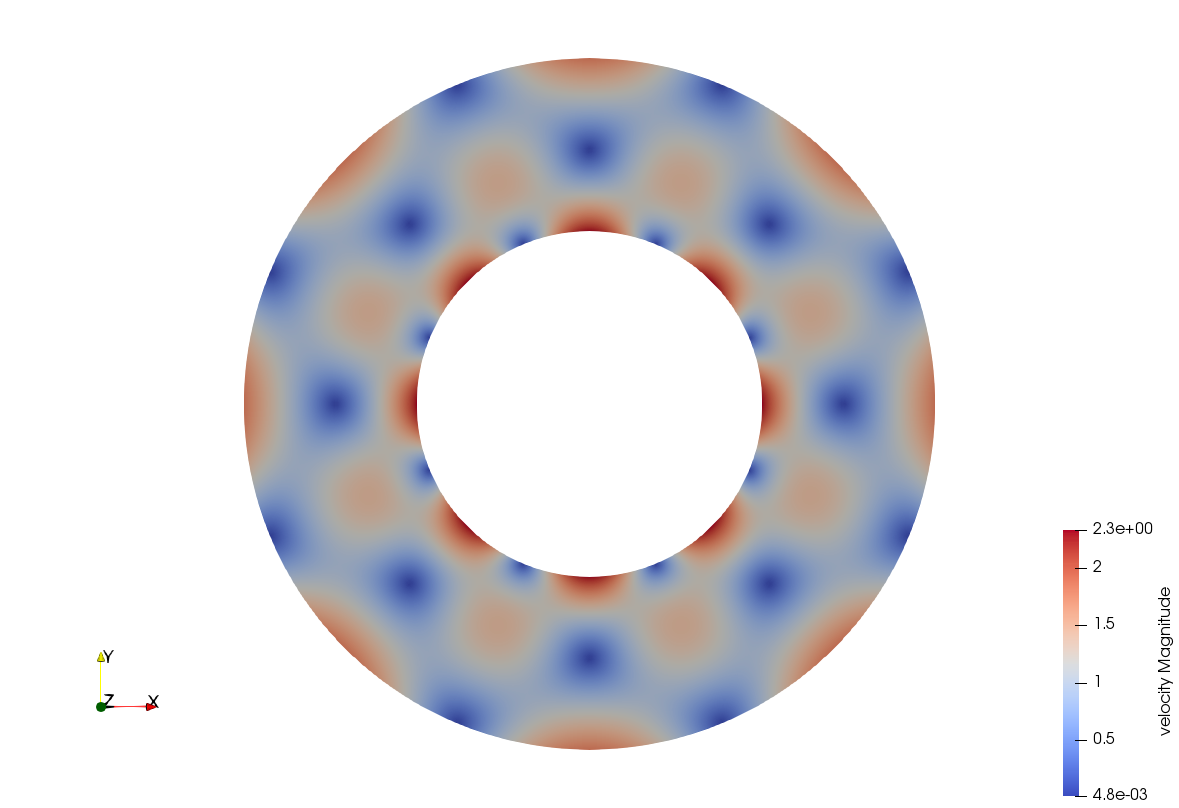
\includegraphics[width=6cm]{python_codes/fieldstone_09/velocity}

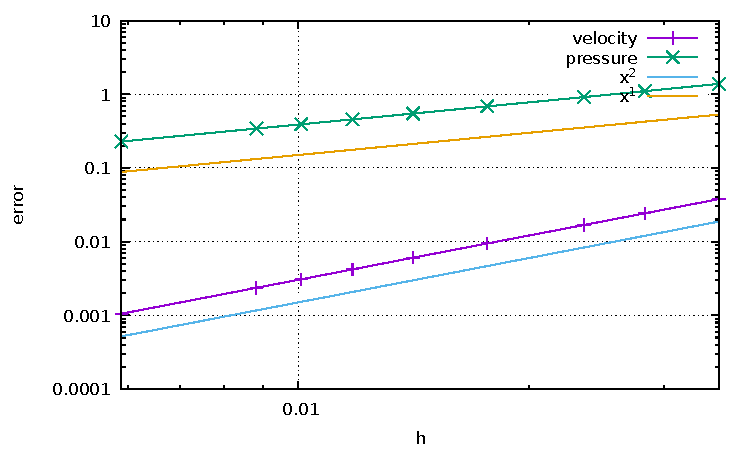
\includegraphics[width=16cm]{python_codes/fieldstone_09/errors}

